\documentclass[10pt]{standalone}
\usepackage{amsmath}
\usepackage{amssymb}
\usepackage{pgf,tikz}
\usepackage{mathrsfs}
\usetikzlibrary{arrows,calc,positioning,shapes.symbols,shapes.geometric,shapes.misc}
\pagestyle{empty}
\usepackage{siunitx}


\begin{document}

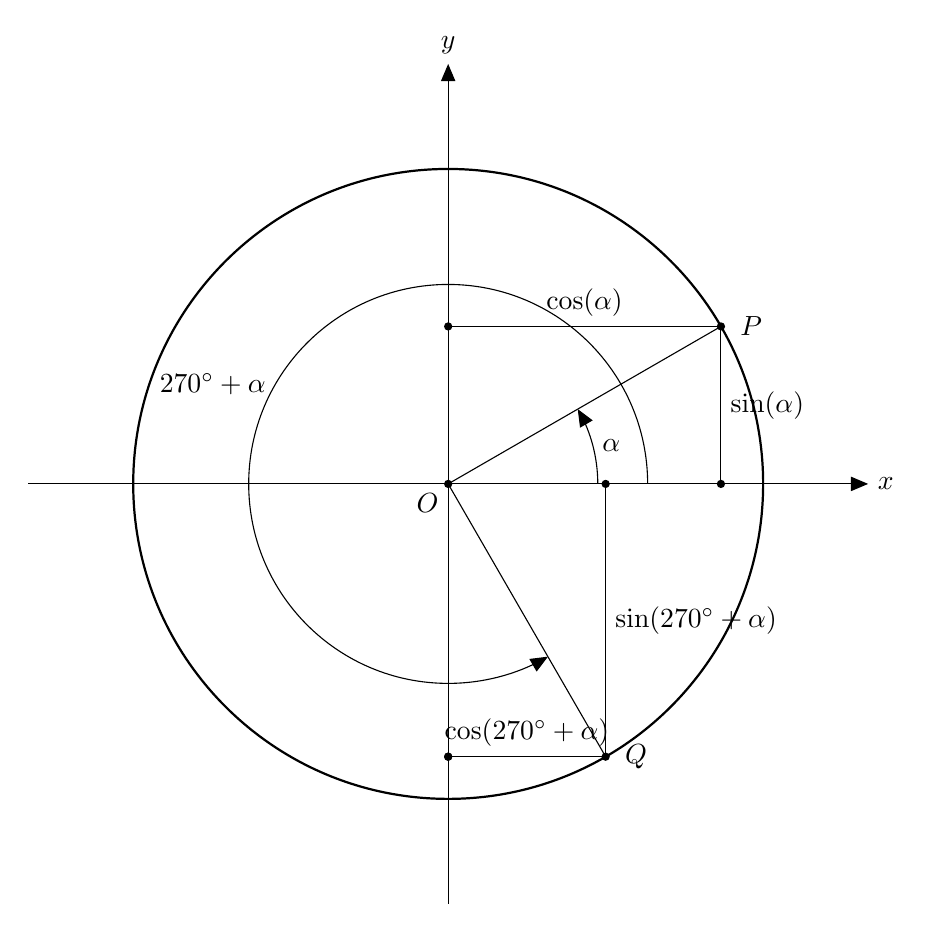
\begin{tikzpicture}[>=triangle 45]
% draw the coordinates

\pgfmathsetmacro{\raggio}{4};
\pgfmathsetmacro{\pangolo}{30};
\pgfmathsetmacro{\sangolo}{{270+\pangolo}};
\pgfmathsetmacro{\mraggio}{\raggio/3};
\pgfmathsetmacro{\sraggio}{1.9*\raggio};
% draw the unit circle
\draw[->] (0,-\raggio-\mraggio) -- (0,\raggio+\mraggio) node[above,fill=white] {$y$};
\draw[->] (-\raggio-\mraggio,0) -- (\raggio+\mraggio,0) node[right,fill=white] {$x$};
\draw[thick] (0,0) circle(\raggio);
\coordinate [label= below left:$O$] (OO)at(0,0);
\coordinate (P)  at ({\raggio*cos(\pangolo},{\raggio*sin(\pangolo});
\coordinate (PX)  at ({\raggio*cos(\pangolo},0);
\coordinate (PY)  at (0,{\raggio*sin(\pangolo});
\coordinate (Q)  at ({\raggio*cos(\sangolo},{\raggio*sin(\sangolo});
\coordinate (QX)  at ({\raggio*cos(\sangolo},0);
\coordinate (QY)  at (0,{\raggio*sin(\sangolo});
\coordinate (M)  at (0,{\raggio*sin(\sangolo});
\node at (P) [label=right:$P$]{};
\node at (Q) [label=right:$Q$]{};
\fill [color=black] (OO) circle (1.5pt);
\fill [color=black] (P) circle (1.5pt);
\fill [color=black] (PX) circle (1.5pt);
\fill [color=black] (PY) circle (1.5pt);
\fill [color=black] (M) circle (1.5pt);
\fill [color=black] (Q) circle (1.5pt);
\fill [color=black] (QX) circle (1.5pt);
\fill [color=black] (QY) circle (1.5pt);
%\draw[->] {(\sraggio/2.5},0 ) arc (0:\pangolo:\sraggio/2.5) node[above] {$\arco$};
\draw(P)--(PY) node[midway,above] {$\cos(\alpha)$};
\draw(Q)--(QY) node[midway,above] {$\cos(\ang{270}+\alpha)$};
\draw(P)--(PX) node[midway,right] {$\sin(\alpha)$};
\draw(Q)--(QX)node[midway,right] {$\sin(\ang{270}+\alpha)$};
\draw [->] (0:\sraggio/3) arc (0:\sangolo:\sraggio/3);
	\draw (\sangolo/2:\sraggio/3) node[left] {$\ang{270}+\alpha$};
\draw [->] (0:\sraggio/4) arc (0:\pangolo:\sraggio/4);
	\draw (\pangolo/2:\sraggio/4) node[right] {$\alpha$};
\draw(OO)--(P);
\draw(OO)--(Q);
\end{tikzpicture}

\end{document}